\chapter{Proposed Methods}

\section{Diversified Class Activation Maps (\divcam)}
\label{sec:divcam}

\begin{figure}[t]
    \centering
    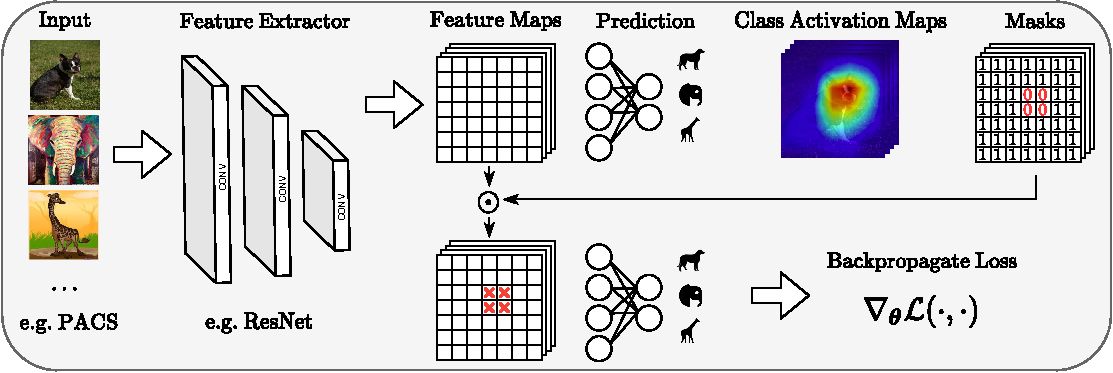
\includegraphics[width=\textwidth]{Figures/Chapter4/model_figure-cropped.pdf}
    \caption{Visualization of the \divcam training process}
    \label{fig:divcam-overview}
\end{figure}


In \Cref{sec:RSC} we introduce the concept of Representation Self-Challenging for domain generalization while in \Cref{sec:CAMs} class activation maps, and specifically Grad-CAM gets introduced. It is quite easy to see that the importance scores $ \Tilde{\mathbf{g}}_{\mathbf{z},c}^k$ in Grad-Cam from \Cref{eq:grad_cam_importance} are a generalization of the spatial mean $\featurega$ used in Channel-Wise RSC from \Cref{eq:ChannelRSCavg}. The spatial mean $\featurega$ only computes the gradient with respect to the features for the most probable class while the importance scores $ \Tilde{\mathbf{g}}_{\mathbf{z},c}^k$ are formulated theoretically for all possible classes but similarly compute the gradient with respect to the feature representation. Both perform spatial average pooling.  

Despite the effectiveness of the model, we believe the approach of \citet{huang2020selfchallenging} does not fully exploit the relation between a feature vector and the actual content of the image. We argue (and experimentally demonstrate) that we can directly use CAMs to construct the self-challenging task. In particular, while the raw target gradient represents the significance of each channel in each spatial location for the prediction, CAMs allow us to better capture the actual importance of each image region. Thus, performing the targeted masking on highest CAM values means explicitly excluding the most relevant \emph{region} of the image that where used for the prediction, forcing the model to focus on other (and interpretable) visual cues for the recognizing the object of interests. 

Therefore, as an intuitive baseline, we propose Diversified Class Activation Maps (\divcam), combining the two approaches as shown in \Cref{alg:ActivationMasking} or visualized on a high level in \Cref{fig:divcam-overview}. For that, during each step of the training procedure, we extract the features, compute the gradients with respect to the features as in \Cref{eq:gz}, and perform spatial average pooling to yield $\featurega$ according to \Cref{eq:ChannelRSCavg}. Our method deviates from Channel-Wise RSC by next computing class activation maps $\mathbf{M}_c \in \mathbb{R}^{H_\mathbf{z} \times W_\mathbf{z} \times 1}$ according to \Cref{eq:Map} for the ground truth class label.
\begin{equation}
\label{eq:Map}
    \mathbf{M}_c = \mathtt{max}(0,\sum_{k=1}^K\Tilde{\mathbf{g}}_{\mathbf{z},c}^k \mathbf{z}^k)
\end{equation}
Based on these maps and similar to \Cref{eq:Masking}, we compute a mask $\mathbf{m} \in \mathbb{R}^{H_\mathbf{z} \times W_\mathbf{z} \times 1}$ for the Top-$p$ percentile of map activations as: 
\begin{equation}
\mathbf{m}_{c,i,j}=\left\{\begin{array}{ll}
0, & \text { if } \quad \mathbf{M}_{c, i,j} \geq q_{p} \\
1, & \text { otherwise }
\end{array}\right.
\label{eq:MaskMap}
\end{equation}
As class activation maps and the corresponding masks are averaged along the channel dimension to be specific for each spatial location, we duplicate the mask along all channels to yield a mask with the same size of the features $\mathbf{m} \in \mathbb{R}^{H_\mathbf{z} \times W_\mathbf{z} \times K}$ which can directly be multiplied with the features to mask them and to regularized the training procedure:
\begin{equation}
\label{eq:mutate}
\Tilde{\mathbf{z}} = \mathbf{m} \odot \mathbf{z},
\end{equation}
where $\odot$ is the Hadamard product. The new feature vector $\Tilde{\mathbf{z}}$ is used as input to the classifier $w$ in place of the original $\mathbf{z}$ to regularize the training procedure. For the masked features, we compute the Cross-Entropy Loss from \Cref{eq:cross_entropy} and backpropagate the gradient of the loss to the whole network to update the parameters.

Intuitively, constantly applying this masking for all samples within each batch disregards important features and results in relatively poor performance as the network isn't able to learn discriminative features in the first place. Therefore, applying the mask only for certain samples within each batch as mentioned by \citet[Secton~3.3]{huang2020selfchallenging} should yield a better performance. For convenience, we call this process \emph{mask batching}. On top of that, one could schedule the mask batching with an increasing factor (\eg linear schedule) such that masking gets applied more in the later training epochs where discriminative features have been learned. We apply the mask only if the sample $n$ is within the $(100-b)\mathrm{th}$ percentile of confidences for the correct class and reset the mask otherwise by setting each spatial location $(i,j)$ back to $1$:
\begin{equation}
    \mathbf{m}^n_{c,i,j}=\left\{\begin{array}{ll}
1, & \text { if } \quad \mathbf{c}^n \leq q_{b} \\
-, & \text { otherwise }
\end{array}\right.
\label{eq:MaskingReversion}
\end{equation}
 where $ \mathbf{c}^n$ is is the confidence on the ground truth for sample $n$. This procedure enforces that masks only get applied to samples which are already classified well enough such that the network can now focus on other discriminative properties. For our full ablation study on applying the masks within each batch, please see \Cref{sec:ablation_study_batching}.

To try and improve the effectiveness of our CAM-based regularization approach, we can borrow some practices from the weakly-supervised object localization literature. In particular, we explore the use of Homogeneous Negative CAMs (HNC) \citep{sun2020fixing} and Threshold Average Pooling (TAP) \citep{Bae2020RethinkingCAM}. Both methods improve the performance of ordinary CAMs and focus them better on the relevant aspects of an image. See \Cref{sec:abl-masks} for an evaluation of these variants.

\subsection{Global Average Pooling bias for small activation areas}
According to \citet{Bae2020RethinkingCAM}, one problem of traditional class activation maps is that the activated areas for each feature map differ by the respective channels because these capture different class information which isn't properly reflected in the global average pooling operation. Since every channel is globally averaged, smaller feature activation areas result in smaller globally averaged values despite a similar maximum activation value. This doesn't necessarily mean that one of the features is more relevant for the prediction, but can simply be caused by a smaller activation area. To combat the smaller value for the prediction, the weight $w_{k,c}$ corresponding to the smaller value, is often trained to be higher when comparing two channels \citep{Bae2020RethinkingCAM}. Instead of the global average pooling operation, they propose \emph{Threshold Average Pooling} (TAP). When adapting their approach for our notation, we receive \Cref{eq:tap} where $\tau_{t a p} = \theta_{tap} \cdot \mathtt{max}(\Tilde{\mathbf{z}}^k)$ with $\theta_{tap} \in [0,1)$ as a hyperparameter and $p^k_{tap}$ denotes the scalar from the $k$-th channel of $\mathbf{p}_{tap}$ as it is a $k$-dimensional vector. 
\begin{equation}
\label{eq:tap}
p^k_{tap} =\frac{\sum_{i=1}^{H_\mathbf{z}} \sum_{j=1}^{W_\mathbf{z}} \mathds{1}\left(\Tilde{\mathbf{z}}^k_{i,j} > \tau_{t a p}\right) \Tilde{\mathbf{z}}^k_{i,j}}{\sum_{i=1}^{H_\mathbf{z}} \sum_{j=1}^{W_\mathbf{z}} \mathds{1}\left(\Tilde{\mathbf{z}}^k_{i,j} > \tau_{t a p}\right)}
\end{equation}
When incorporating this into \divcam, this results in changing the global average pooling after the last convolutional layer in the ResNet architecture to a threshold average pooling. Generally, this plug-in replacement can be seen as a trade-off between \emph{global max pooling} which is better at identifying the important activations of each channel and \emph{global average pooling} which has the advantage that it expands the activation to broader regions, allowing the loss to backpropagate.

\begin{algorithm}[t]
    \SetAlgoLined
    \SetKwInOut{Input}{Input}
    \Input{Data $\mathbf{X}, \mathbf{Y}$ with $\mathbf{x}_i \in \mathbb{R}^{H \times W \times 3}$, drop factor $p,b$, epochs $T$}
    \BlankLine
    \While{$epoch \leq T$}{
        \For{every batch $\mathbf{x}, \mathbf{y}$}{
            Extract features $\mathbf{z} = \phi(\mathbf{x})$ \tcp*[r]{$\mathbf{z}$ has shape  $\mathbb{R}^{H_\mathbf{z} \times W_\mathbf{z} \times K} $}
            Compute $\mathbf{g}_{\mathbf{z},c}$ with \Cref{eq:gz}\;
            Compute $\Tilde{\mathbf{g}}_{\mathbf{z},c}^k$ with \Cref{eq:ChannelRSCavg} \tcp*[r]{$\featurega$ has shape $\mathbb{R}^{1 \times 1 \times K}$}
            Compute $\mathbf{M}_c$ with \Cref{eq:Map} \tcp*[r]{$\mathbf{M}$ has shape $\mathbb{R}^{H_\mathbf{z} \times W_\mathbf{z} \times 1}$}
            Compute $\mathbf{m}_{c,i,j}$ with \Cref{eq:MaskMap} \;
            Repeat mask along channels \tcp*[r]{Afterwards $\mathbf{m}$ has shape $\mathbb{R}^{H_\mathbf{z} \times W_\mathbf{z} \times K}$}
            Adapt $\mathbf{m}_{c,i,j}$ with \Cref{eq:MaskingReversion} \;
            Compute $\Tilde{\mathbf{z}}$ with \Cref{eq:mutate} \;
            Backpropagate loss $\mathcal{L}_{ce}(w(\Tilde{\mathbf{z}}), \mathbf{y})$ \;
            }
    }
\caption{Diversified Class Activation Maps (\divcam)}
\label{alg:ActivationMasking}
\end{algorithm}

\subsection{Smoothing negative Class Activation Maps}
Based on the analysis of \citet{sun2020fixing}, negative class activation maps, \ie the class activation maps for classes other than the ground truth, often have false activations even when they are not present in an image. To solve this localization error, they propose a loss function which adds a weighted \emph{homogeneous negative CAM} (HNC) loss term to the existing Cross-Entropy loss. This is shown in \Cref{eq:hnc} where $\lambda_1$ controls the weight of the additional loss term. 
\begin{equation}
\label{eq:hnc}
\mathcal{L}_{neg} =\mathcal{L}_{ce}(\mathbf{y}, w(\Tilde{\mathbf{z}}))+\lambda_1 \mathcal{L}_{hnc}(\mathbf{y}, \boldsymbol{M})
\end{equation}
\citet{sun2020fixing} propose two approaches for implementing $\mathcal{L}_{hnc}$ in their work, both operating on the Top-$k$ most confident negative classes. The first one is based on the mean squared error which suppresses peak responses in the CAMs, while the second one utilizes the Kullback–Leibler (KL) divergence trying to minimize the difference between negative CAMs and an uniform probability map. Since they report similar performance for these variants and the KL loss applies a comparably smoother penalty, we use the KL divergence for our method:
\begin{equation}
\label{eq:hnc-kl}
\mathcal{L}_{hnc}(\mathbf{y}, \boldsymbol{M})=\sum_{c \in J^{\prime}_>} D_{K L}\left(\boldsymbol{U} \| \boldsymbol{M}_{c}^{\prime}\right).
\end{equation}
Here, $J^{\prime}_>$ is the set of Top-$k$ negative classes with the highest confidence score, $\boldsymbol{U} \in \mathbb{R}^{H_\mathbf{z} \times W_\mathbf{z}}$ is a uniform probability matrix with all elements having the value $(H_\mathbf{z}W_\mathbf{z})^{-1}$, and $\boldsymbol{M}_{c}^{\prime} = \sigma(\boldsymbol{M}_{c})$ is a probability map produced by applying the softmax function $\sigma$ to each negative class activation map $\boldsymbol{M}_{c}$. Plugging in the definition of the KL divergence and removing the constant as in \Cref{eq:kl-simplification} finally results in a simplified version as
\Cref{eq:hnc-kl-simple}.
\begin{equation}
\label{eq:kl-simplification}
D_{K L}\left(\boldsymbol{U} \| \boldsymbol{M}_{c}^{\prime}\right)=\sum_{i=1}^{H_\mathbf{z}} \sum_{j=1}^{W_\mathbf{z}} \boldsymbol{U}_{i,j} \cdot \log \left( \frac{\boldsymbol{U}_{i,j}}{\boldsymbol{M}_{c, i, j}^{\prime}} \right) =\text { const }-\frac{1}{H_\mathbf{z} W_\mathbf{z}} \sum_{i=1}^{H_\mathbf{z}} \sum_{j=1}^{W_\mathbf{z}} \log \left(\boldsymbol{M}_{c, i, j}^{\prime}\right)
\end{equation}
Generally, with this approach, we add two hyperparametes in the form of the weighting parameter $\lambda$ and the cut-off number $k$ for the Top-$k$ negative classes.
\begin{equation}
\label{eq:hnc-kl-simple}
    \mathcal{L}_{hnc}(\mathbf{y}, \boldsymbol{M})= -\frac{1}{H_\mathbf{z} W_\mathbf{z}} \sum_{c \in J^{\prime}_>} \sum_{i=1}^{H_\mathbf{z}} \sum_{j=1}^{W_\mathbf{z}} \log \left(\boldsymbol{M}_{c, i, j}^{\prime}\right)
\end{equation}
Since we use Grad-CAMs instead of ordinary CAMs in \divcam, na\"{i}vely applying this would require computing the gradient for every negative class $c$ in the set $J^\prime_>$ which would result in computing \Cref{eq:hnc-kl-grad-cam} where $y_c$ is the confidence of the negative class. 
\begin{equation}
\label{eq:hnc-kl-grad-cam}
    \mathcal{L}_{hnc}(\mathbf{y}, \boldsymbol{M})= -\frac{1}{H_\mathbf{z} W_\mathbf{z}} \sum_{c \in J^{\prime}_>} \sum_{i=1}^{H_\mathbf{z}} \sum_{j=1}^{W_\mathbf{z}} \log \left( \sigma \left(\mathtt{max}\left(0,\sum_{k=1}^K\left(\frac{1}{H_\mathbf{z}W_\mathbf{z}} \sum_{i=1}^{H_\mathbf{z}} \sum_{j=1}^{W_\mathbf{z}} \frac{\partial y_c}{\partial \mathbf{z}_{i,j}^k}\right)^k \mathbf{z}^k\right)\right)\right)
\end{equation}
To speed up the training for tasks with a large number of classes, we approximate the loss by summing the negative class confidences before backpropagating as shown in \Cref{eq:hnc-kl-grad-cam-approx}. This amounts to considering all negative classes within $J^\prime_>$ as one negative class. 
\begin{equation}
\label{eq:hnc-kl-grad-cam-approx}
    \widehat{\mathcal{L}}_{hnc}(\mathbf{y}, \boldsymbol{M})= -\frac{1}{H_\mathbf{z} W_\mathbf{z}} \sum_{i=1}^{H_\mathbf{z}} \sum_{j=1}^{W_\mathbf{z}} \log \left( \sigma \left(\mathtt{max}\left(0,\sum_{k=1}^K\left(\frac{1}{H_\mathbf{z}W_\mathbf{z}} \sum_{i=1}^{H_\mathbf{z}} \sum_{j=1}^{W_\mathbf{z}} \frac{\partial \sum_{c \in J^{\prime}_>} y_c}{\partial \mathbf{z}_{i,j}^k}\right)^k \mathbf{z}^k\right)\right)\right)
\end{equation}
To finally implement this into \divcam, we simply substitute the current loss $\mathcal{L}_{ce}(\mathbf{y}, w(\Tilde{\mathbf{z}}))$ in line $12$ from \Cref{alg:ActivationMasking} with \Cref{eq:hnc} where $\mathcal{L}_{hnc}(\mathbf{y}, \boldsymbol{M})$ is implemented through our approximation $\widehat{\mathcal{L}}_{hnc}(\mathbf{y}, \boldsymbol{M})$ given in \Cref{eq:hnc-kl-grad-cam-approx}. 


Next, we can try to utilize more domain information in \divcam by aligning distributions of class activation maps produced by the same class across domains. Intuitively, we want their distributions to align as close as possible such that we cannot identify which domain produced which class activation map. For that, we can utilize some methods previously introduced in \Cref{sec:invariant_features}, in particular we explore minimizing the sample maximum mean discrepancy introduced in \Cref{eq:mmd} and using a conditional domain adversarial neural network (CDANN). See \Cref{sec:abl-masks} for an evaluation of these variants.

\subsection{Conditional Domain Adversarial Neural Networks}
We combine the domain adversarial neural network (CDANN) approach, originally introduced by \citet{LiGTLT18}, with \divcam to align the distributions of CAMs across domains. For that, we try to predict the domain to which a class activation map belongs by passing it to a multi-layer perceptron $\omega$. We compute the cross entropy loss between the predictions and the domain ground truth $\mathbf{d}$ and weight it for each sample by the occurrence probability of the respective class.
After weighting, we can sum up all the losses and add it to our overall loss, weighted by $\lambda_2$:
\begin{equation}
\label{eq:adv}
\mathcal{L}_{adv} =\mathcal{L}_{ce}(\mathbf{y}, w(\Tilde{\mathbf{z}}))+\lambda_2 ( \mathcal{L}_{ce}(\mathbf{d}, \omega(\boldsymbol{M})) + \eta \left\|\nabla_{\boldsymbol{M}} \mathcal{L}_{ce}(\mathbf{d}, \omega(\boldsymbol{M}))\right\|_2).
\end{equation}
During each training step, we either update the discriminator, \ie the predictor for the domain, or the generator, \ie the main network including featurizer and classifier. The discriminator loss inherently includes a l2 penalty on the gradients, weighted by $\eta$.


\subsection{Maximum Mean Discrepancy}

Given two samples $\mathbf{x}^{\xi_1}$ and $\mathbf{x}^{\xi_2}$ drawn from two individual, unknown  domain distributions $\mathcal{D}_{\xi_1}$ and $\mathcal{D}_{\xi_2}$, the maximum mean discrepancy (MMD) is given by \Cref{eq:mmd_maps} where $\varphi: \mathbb{R}^{d} \rightarrow \mathcal{H}$ is a feature map and $k(\cdot, \cdot)$ is the kernel function induced by $\varphi(\cdot)$. We consider every distinct pair of source domains $(\xi_u, \xi_v)$, representing training domains $\xi_u$ and $\xi_v$, with $\xi_u\neq \xi_v$ to be in the set $\Gamma$.
\begin{equation}
\label{eq:mmd_maps}
    \mathcal{L}_{dist} =\sum_{\xi_u,\xi_v \in \Gamma}\left\|\mathbb{E}_{\mathbf{x}^{\xi_u} \sim \mathcal{D}_{\xi_u}}[\varphi(\mathbf{x}^{\xi_u})]-\mathbb{E}_{\mathbf{x}^{\xi_v} \sim \mathcal{D}_{\xi_v}}[\varphi(\mathbf{x}^{\xi_v})]\right\|_{\mathcal{H}}
\end{equation}
In simpler terms, we map samples into a reproducing kernel Hilbert space $\mathcal{H}$, and compute their mean differences within the RKHS. This loss pushes samples from different domains, which represent the same class, to lie nearby in the embedding space. According to \citet{SriperumbudurFGLS09}, this mean embedding is injective, \ie arbitrary distributions are uniquely represented in the RKHS, if we use a characteristic kernel. For this work, we choose the gaussian kernel shown in \Cref{eq:gaussian_kernel} which is a well-known characteristic kernel.
\begin{equation}
\label{eq:gaussian_kernel}
    k(x,x') = \exp \left(-\frac{\|x-x'\|^{2}}{2 \sigma^{2}}\right)
\end{equation}
Since the choice of kernel function can have a significant impact on the distance metric, we adopt the approach of \citet{LiPWK18} and use a mixture kernel by averaging over multiple choices of $\sigma$ as already implemented in \domainbed. This gets incorporated into our loss function weighted by $\lambda_3$ with:
\begin{equation}
    \mathcal{L}_{mmd} = \mathcal{L}_{ce}(\mathbf{y}, w(\Tilde{\mathbf{z}}))+\lambda_3 \mathcal{L}_{dist}.
\end{equation}
With this approach, we inherently align the computed masks by aligning the individual samples from different domains, aiming at producing domain invariant masks. 

\section{Prototype Networks for Domain Generalization}
\label{sec:prototype_networks}

Another approach to combine explainability methods with the task of domain generalization is to use the prototype approach outlined in \Cref{sec:prototypes}. In particular, we can directly adapt the approach of \citet{ChenLTBRS19} as a baseline where we associate each class with a pre-defined number of prototypes. The cluster and separation losses from \Cref{eq:prototype_losses} ensure that each prototype resembles a prototypical attribute for the associated class and we minimize them according to \Cref{eq:min_prototypes}.

\begin{figure*}[t]
    \centering
    
\includegraphics[width=\textwidth, height=5cm]{Figures/img-placeholder.png}
    \caption{Domain-agnostic Prototype Network}
    \label{fig:domain_prototype_network}
\end{figure*}

For our application scenario, this prototype layer is used after the domain-agnostic featurizer $\phi$ and operates on the features like illustrated in \Cref{fig:domain_prototype_network}. As each prototype is trained with data from all training domains $\Xi$, they become inherently domain agnostic. This baseline uses a joint classifier $w$ to output the final prediction which operates on the maximum similarity for all the prototypes and \emph{some} latent patch. Similar to \citet{ChenLTBRS19}, we preface the prototype layer with two convolutional layers with kernel size $1$, a ReLU function between them, and finally a sigmoid activation function. We observe that having roughly $100$ initial update steps where only these in-between layers are trained is crucial for competitive performance. We anticipate that these steps are used to adapt the untrained convolutional weights to the image statics imposed by the pre-trained backbone.\footnote{Further implementation details can be found here: \url{https://github.com/SirRob1997/DomainBed/}}


\subsection{Ensemble Prototype Network}
Following the intuition provided by works that utilize model ensembling, which have been described in \Cref{sec:model_ensembling}, we can use domain information by up-scaling the network to use a prototype layer for each domain separately. For the PACS dataset, this would correspond to having three prototype layers, one for each training domain \eg a photo, art, and cartoon prototype layer when predicting sketch images. Each prototype layer is only trained with images from their corresponding domain.

As shown in \Cref{fig:ensemble_prototype_network}, we associate each domain with both a prototype layer and a classifier which takes similarity scores of that domain's prototypes as input. During training, we only feed images of the associated domain to the respective prototype layer and classifier to enforce this domain correspondence. The aggregation weights of the final linear layer are set to a one-hot encoding representing the correct domain. During testing, we can then feed the new unseen domain to each domain prototype layer, allowing each domain's prototypes to influence the final prediction. 

There exist multiple strategies for setting the aggregation weights during this stage. The most simple version is to set the influence of each domain uniform, \ie if we have three training domains the connections from each domain would have the weight $\frac{1}{3}$ such that each domain has the same influence on the final prediction. Our second approach is to jointly train a domain predictor to output the weights for the aggregation layer which can either be used both, during training and testing, or only during testing, similar to what is done by \citet{ManciniBC018}. This method allows for a more flexible aggregation of the separated predictions coming from the different prototype layers, enabling the network to put more emphasis on the relevant domain prototypes.  

\begin{figure*}[t]
    \centering
    
\includegraphics[width=\textwidth, height=5cm]{Figures/img-placeholder.png}
    \caption{Ensemble Prototype Network}
    \label{fig:ensemble_prototype_network}
\end{figure*}

Lastly, we also experiment with an ensemble variant that is specific to prototype layers. Instead of only pre-defining a number of prototypes for each class in the domain agnostic prototype layer outlined in \Cref{sec:prototype_networks}, we can also pre-define domain correspondence for each prototype. Training is then done by passing each domain separately to the prototype layer and masking the overall prototype outputs if they do not correspond to the current environment. The cluster and separation losses are adapted to an average over the individual environments as:
\begin{alignat}{3}
\label{eq:prototype_losses_domain}
    \mathcal{L}_{\mathrm{clst}} &= \frac{1}{s} \sum_{\env \in \envs} &&\frac{1}{n_\env} \sum_{i=1}^{n_\env} \min_{j: \prot\in \prots_{\yyi}^\env} \min_{\zpatch \in \text{patches}(\zz^\env)} \left\|\zpatch - \prot\right\|^2_2\\
    \mathcal{L}_{\mathrm{sep}} &= \frac{1}{s} \sum_{\env \in \envs}-&&\frac{1}{n_\env} \sum_{i=1}^{n_\env} \min_{j: \prot \notin \prots_{\yyi}^\env} \min_{\zpatch \in \text{patches}(\zz^\env)} \left\|\zpatch - \prot\right\|^2_2,
\end{alignat}
where $\prots_{\yyi}^\env$ denotes the prototypes associated with the specific class \emph{and} environment while $\zz^\env$ denotes the latent representation of an image corresponding to the current domain. This ensemble variant inherently removes the need for setting appropriate aggregations weights as prototype activations are simply masked during training while during testing all prototypes are kept, allowing each prototype from each source domain to influence the prediction.  

While all of these ensemble variants \emph{should} work given the intuition from previous works that have been using model ensembles for learned domain-specific latent spaces, we observe that these assumptions do \emph{not} hold for prototype networks based on our additional experiments of the proposed variants. For us, any prototype ensemble was consistently outperformed by one domain-agnostic prototype layer. 

\subsection{Diversified Prototypes (\prodrop)}

To improve upon the domain-agnostic prototype layer, we analyze the best performing hyperparameters (oracle-validation) for their learned, pairwise prototype $\ell_2$-distance as well as the cosine distance $\cdistance$ which for any two prototypes $\prot$ and $\proti_i$ are given by:
\begin{alignat}{3}
\label{eq:pairwise_prot_distances}
    &\ell_2 &&= &&\left\|\proti_i - \prot  \right\|_2\\ 
    &\cdistance &&= 1- &&\frac{\proti_i\prot}{\left\|\proti_i \right\|_2 \left\|\prot \right\|_2} .
\end{alignat}
Through the $\ell_2$-distance we can grasp the euclidean distance between any two prototypes while the cosine distance $\cdistance \in [0,2]$ is the inverted version of the cosine similarity which is a metric to judge the cosine of the angle between them. Here, we visualize the cosine distance instead of the cosine similarity to match the color-scheme of the $\ell_2$-distance \ie low values resemble closeness. 


\begin{figure}[t]
    \centering
    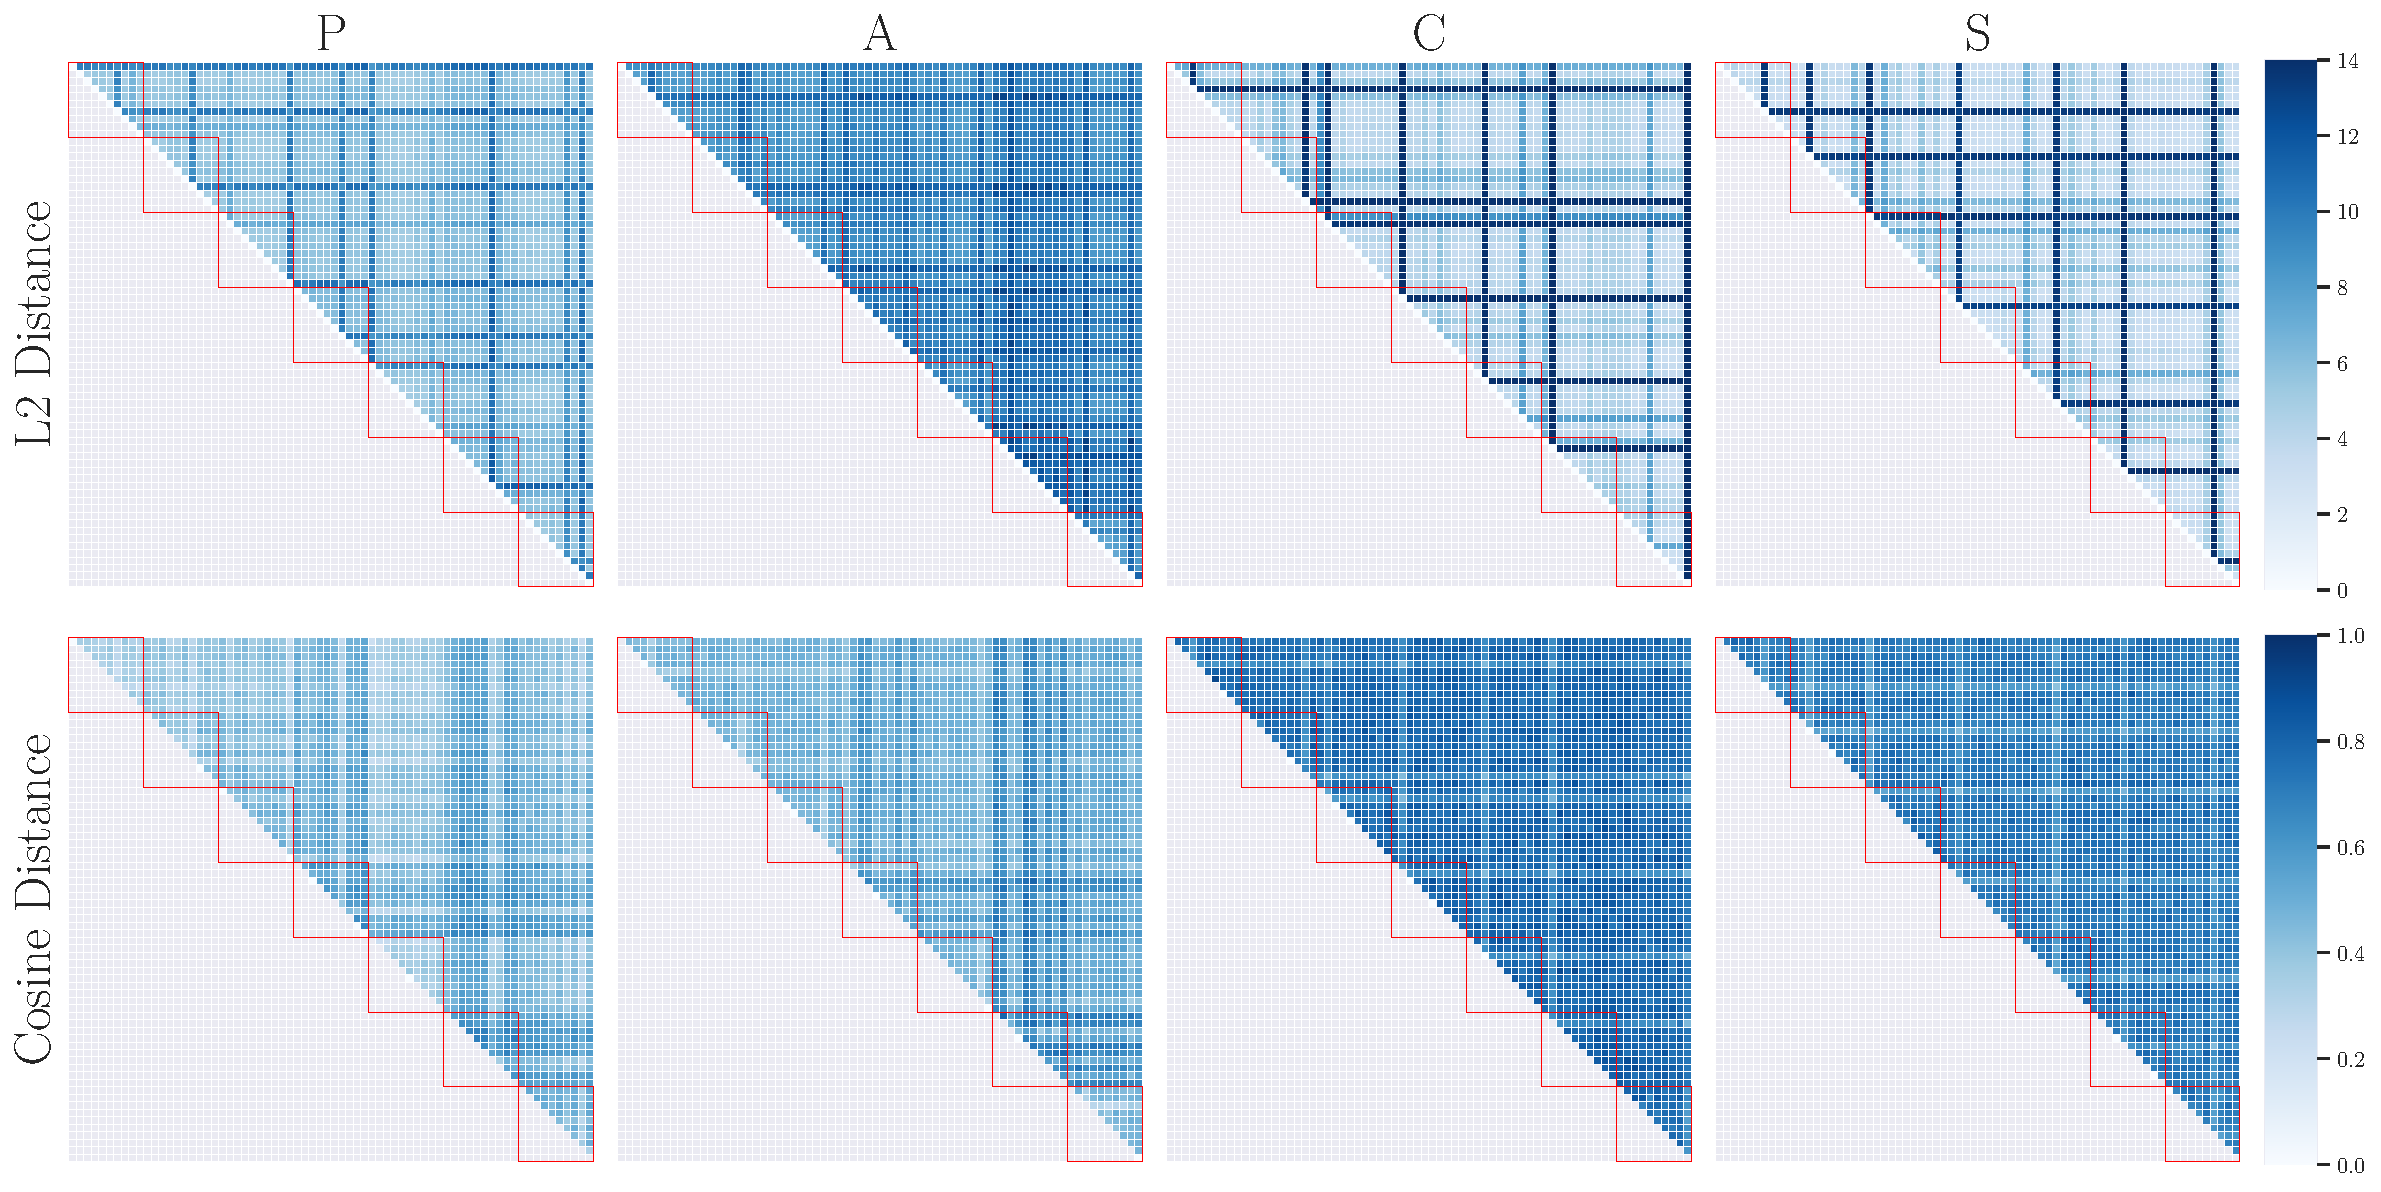
\includegraphics[width=\textwidth]{Figures/Chapter4/2021-01-21-ProDropIncorrectWeight-1.0SAVEResNet18oracle_validation_trial1.pdf}
    \caption[Second data split pairwise prototype distances with $w_{c,j} = -1.0$] {Best-performing pairwise learned prototype $\ell_2$-distance (top) and cosine distance $\cdistance$ (bottom) with negative weight $w_{c,j} = -1.0\; \forall j: \prot \notin \prots_c$ for each testing domain. Red squares denote prototype class correspondence for the $7$ different classes in the PACS dataset. No self-challenging is applied and colormap bounds are adjusted per metric for visualization purposes. Second data split.}
    \label{fig:pw_distance_trial1}
\end{figure}


The results of this analysis can be seen in \Cref{fig:pairwise_distance} and \Cref{fig:pairwise_distance_sc} for the first data split and a negative weight of $w_{c,j} = -1.0\; \forall j: \prot \notin \prots_c$ but we also show the same plots for $w_{c,j} = 0.0$ and the two additional data splits in \Cref{sec:additional_distances}. As both of the used metrics are symmetric, only the upper triangle is visualized. We observe that depending on the data split and negative weight, the model sometimes converges to having one or two prototypes per class that have a large $\ell_2$ distance while many of the other prototypes are close. Striking examples for this behavior can be seen in \Cref{fig:pairwise_distance} for the sketch domain or in \Cref{fig:pw_distance_trial1} for the sketch and cartoon domain. This observation suggests, that in these scenarios the model fails to properly use all of the available prototypes and only relies on a significantly reduced subset per class, not training the other prototypes. In relation to the cosine distance, however, we can often observe that exactly these prototypes with a high pairwise $\ell_2$-distance to all the other prototypes have a slightly lower cosine distance. Such behavior can be seen for example in \Cref{fig:pairwise_distance} in the art and cartoon environment or in \Cref{fig:pw_distance_trial1} for the sketch and cartoon domain. For the most part, many cosine distances tend to be low and more or less uniformly spaced. Nevertheless, we can occasionally identify ``streaking'' patterns in the cosine distances where prototypes for certain classes are well-spaced but they have a larger (or equal) cosine distance to prototypes of other classes. See for example \Cref{fig:pairwise_distance} for the sketch domain, \Cref{fig:pw_distance_0.0_trial1} for the sketch and photo domain, and \Cref{fig:pw_distance_0.0_trial2}  for the sketch and cartoon domain.

From a design standpoint, we would like the prototypes within each class to be reasonably well spaced out in the latent space such that they can resemble different discriminiative attributes about each class. That is, we would like the network to utilize all the prototypes and not only rely on a small subset of prototypes or discriminiative features for their prediction. The distances of these prototypes to the prototypes of the other classes, however, should \emph{not} be restrained in any way and should be learned automatically. For example, when predicting different bird species, this allows the network to place similar head prototypes of different classes closer together. The existing cluster and separation losses enforce that each prototype associated with that class is close to at least one latent patch of that class while maximizing the distance to the prototypes of other classes. However, this does not enforce that each prototype associated with that class acts on a different discriminative feature.

One approach to possibly enforce this behavior is to incorporate the self-challenging method previously applied to \divcam to the presented prototype network resulting in a novel algorithm we call \emph{prototype dropping} (\prodrop) which is described in \Cref{alg:ProDrop}. In essence, we extract features by passing our input images to the featurizer $\mathbf{z} = \phi(\mathbf{x})$ and compute the similarity scores for each prototype by passing it to the prototype layer $\unit(\zz)$ with \Cref{eq:prot_layer_function}. Based on these similarity scores, we compute a mask $\mathbf{m}_{c,j}$ for the prototypes of the respective class with the highest activation:
\begin{equation}
\mathbf{m}_{c,j}=\left\{\begin{array}{ll}
0, & \text { if } \quad \unit(\zz) \geq q_{c, p}\quad \forall j: \prot \in \prots_c \\
1, & \text { otherwise }.
\end{array}\right.
\label{eq:ProDropFeatureMask}
\end{equation}
We also apply the mask batching from \divcam without scheduling which only applies this type of masking for the highest confidence samples on the ground truth. Finally, we can mask the samples using the Hadamard product $\odot$ with:
\begin{equation}
\label{eq:mutate_prodrop}
\mplayer(\zz) = \mathbf{m} \odot \player(\zz).
\end{equation}
In practice, all of these operations can be efficiently implemented using \texttt{torch.quantile}, \texttt{torch.lt}, and \texttt{torch.logical\_or} on small tensors, all of which pose no significant computational overhead.

\begin{algorithm}[t]
    \SetAlgoLined
    \SetKwInOut{Input}{Input}
    \Input{Data $\mathbf{X}, \mathbf{Y}$ with $\mathbf{x}_i \in \mathbb{R}^{H \times W \times 3}$, drop factor $p,b$, epochs $T$}
    \BlankLine
    \While{$epoch \leq T$}{
        \For{every batch $\mathbf{x}, \mathbf{y}$}{
            Extract features $\mathbf{z} = \phi(\mathbf{x})$ \tcp*[r]{$\mathbf{z}$ has shape  $\mathbb{R}^{H_\mathbf{z} \times W_\mathbf{z} \times K} $}
            Compute $\unit(\zz)$ with \Cref{eq:prot_layer_function}\;
            Compute $\mathbf{m}_{c,j}$ with \Cref{eq:ProDropFeatureMask} \;
            Adapt $\mathbf{m}_{c,j}$ with \Cref{eq:MaskingReversion} \;
            Compute $\mplayer(\zz)$ with \Cref{eq:mutate_prodrop} \;
            Backpropagate loss $\mathcal{L}_{ce}(w(\player(\zz)), \mathbf{y}) + \lambda_4 \mathcal{L}_{\mathrm{clst}} + \lambda_5 \mathcal{L}_{\mathrm{sep}}$ \;
            }
    }
\caption{Prototype Dropping (\prodrop)}
\label{alg:ProDrop}
\end{algorithm}

The effect of this approach on the pairwise prototype distances can be seen in \Cref{fig:pairwise_distance_sc} as well as \Cref{sec:additional_distances}. We observe, that even though self-challenging helps to boost the overall performance (see \Cref{sec:abl_self_challenging}), it does not particularly well achieve the previously described desired distance properties and only improves them marginally. Positive effects can be observed in \Cref{fig:pw_distance_trial1-sc} for the sketch and cartoon domain, \Cref{fig:pw_distance_0.0_trial2-sc} for the sketch domain, or \Cref{fig:pw_distance_0.0_trial1-sc} for the cartoon domain.


\begin{figure}[t]
    \centering
    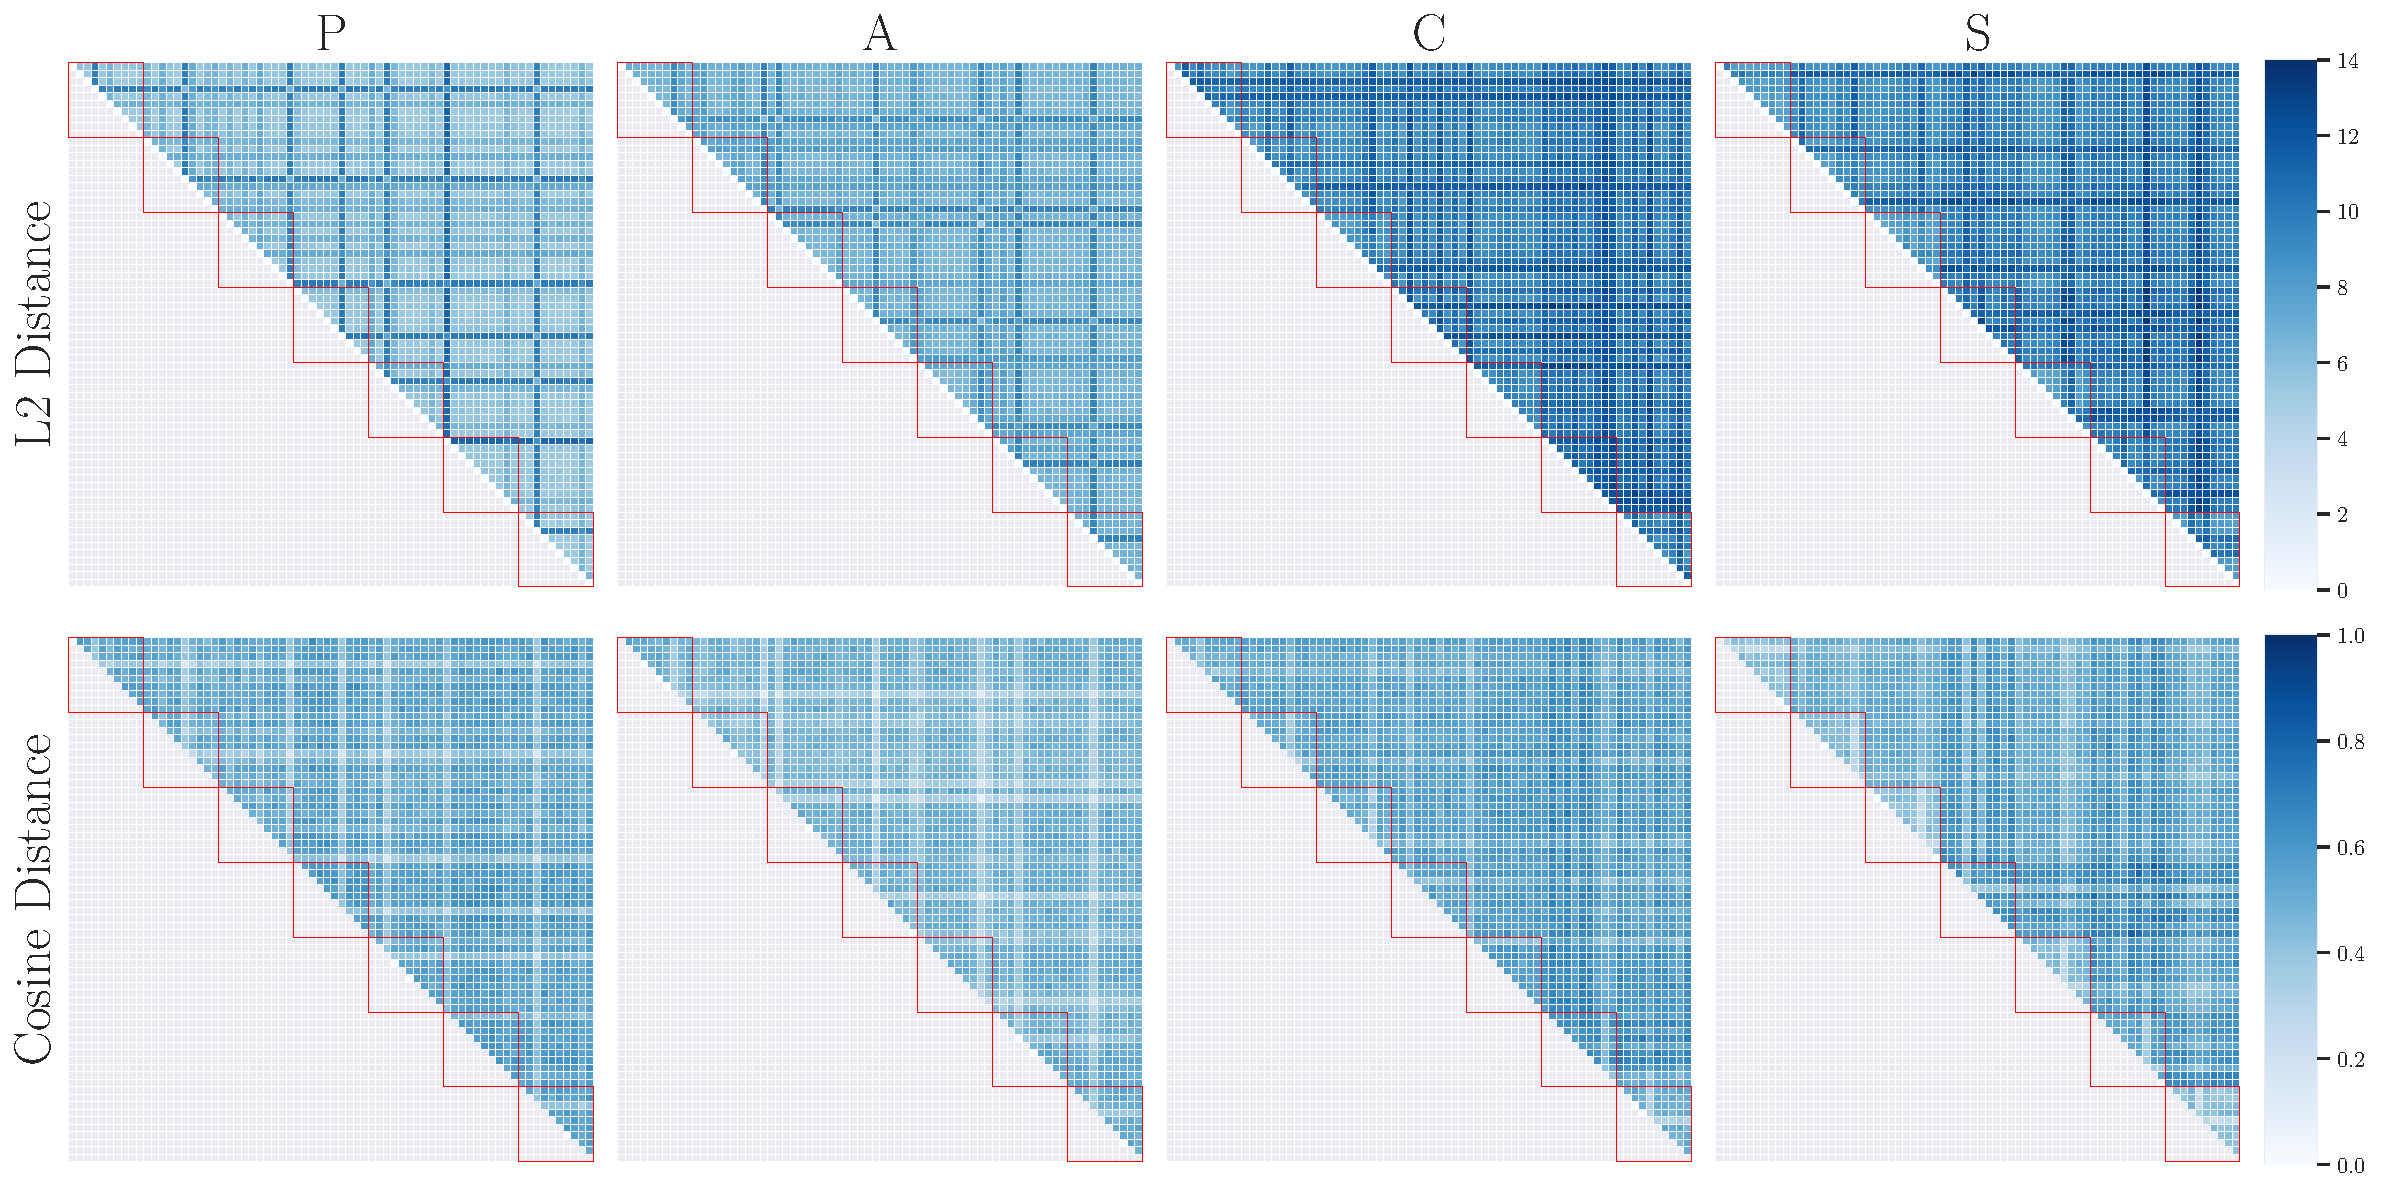
\includegraphics[width=\textwidth]{Figures/Chapter4/2021-01-21-ProDropIncorrectWeight-1.0WithSCdrop_f0.5SAVEResNet18oracle_validation_trial1.pdf}
    \caption[Second data split pairwise self-challenging prototype distances with $w_{c,j} = -1.0$] {Best-performing pairwise learned prototype $\ell_2$-distance (top) and cosine distance $\cdistance$ (bottom) with negative weight $w_{c,j} = -1.0\; \forall j: \prot \notin \prots_c$ for each testing domain. Red squares denote prototype class correspondence for the $7$ different classes in the PACS dataset. Self-challenging is applied and colormap bounds are adjusted per metric for visualization purposes. Second data split.}
    \label{fig:pw_distance_trial1-sc}
\end{figure}

Our second approach to enforce the desired distance structures is to add an additional intra-class prototype loss term $\mathcal{L}_\mathrm{intra}$ which maximizes the intra-class prototoype $\ell_2$- and/or cosine distance weighted by $\lambda_6$. Again, this loss term can \emph{in theory} have a few different definitions. To keep the required hyperparameters to a minimum, we decided to experiment with:
\begin{equation}
\label{eq:intra_loss}
    \mathcal{L}_\mathrm{intra} = \sum_{\proti_i, \prot \in \prots_c} \underbrace{\left\|\proti_i - \prot  \right\|_2 \vphantom{\frac{\proti_i\prot}{\left\|\proti_i \right\|_2 \left\|\prot \right\|_2}}}_{\ell_2-\text{distance}} + \underbrace{ 1-\frac{\proti_i\prot}{\left\|\proti_i \right\|_2 \left\|\prot \right\|_2}}_{\text{cosine distance}},
\end{equation}
where the $\ell_2$-distance and the cosine distance are weighted equally. Since the cosine distance is bounded, this commonly amounts to the $\ell_2$ distance having a higher influence. Performance results for the loss presented in \Cref{eq:intra_loss} are shown in \Cref{sec:intra_loss}. 

Even though we experimented with different weighting of the individual distance metrics as well as the overall loss, we observed no \emph{consistent} performance improvements on top of self-challenging across testing environments and data splits. The observations from \Cref{sec:intra_loss}, \Cref{fig:pw_distance_trial1-sc}, and \Cref{sec:additional_distances} suggest that self-challenging inherently already enforces the desired properties up to the near-optimal extent such that the additional loss term does not provide any consistent further benefits.

\subsection{Influence of the negative weight on the distance metrics}
We also analyze the discrepancies between the distance metrics when comparing $w_{c,j} = -1.0\; \forall j: \prot \notin \prots_c$ and $w_{c,j} = 0.0\; \forall j: \prot \notin \prots_c$ which can be seen in the figures presented in \Cref{sec:additional_distances}. However, from these plots there were no \emph{consistent} trends observable which can be made  

\section{Experiments}
In an effort to improve comparability and reproducability, we use \domainbed \citep{gulrajani2020search} for all ablation studies and experimental results. We compare to all methods currently in \domainbed which includes our provided implementation of \rsc. Further, all experiments show results for both \emph{training-domain validation} which assumes that training and testing domains have similar distributions  and \emph{oracle validation} which has limited access to the testing domain which have been introduced in \Cref{sec:considerations}.

\subsection{Datasets and splits}
Since the size of the validation dataset can have a heavy impact on performance, we follow the design choices of \domainbed and choose $20\%$ of each domain as the validation size for all experiments and ablation studies. Here, we present results for VLCS \citep{FangXR13}, PACS \citep{LiYSH17}, Office-Home \citep{VenkateswaraECP17}, Terra Incognita \citep{BeeryHP18}, and DomainNet \citep{PengBXHSW19}. Although sometimes disregarded in the body of literature for domain generalization, we provide results for three different dataset splits to assess the stability regarding the model selection and to avoid overfitting on one split. 

\subsection{Hyperparameter Distributions \& Schedules}
\label{sec:abl-distr}
For the mask batching ablation study we use \adam \cite{Kingma2015} and the distributions from \Cref{tab:abl-distributions-mask-batching}. When the batch drop factor is scheduled, we use an increasing linear schedule while the learning rate is always scheduled with a step-decay which decays the learning rate by factor $0.1$ at epoch $80/100$.
\begin{table}[!htbp]
    \centering
    \begin{tabular}{lll}
        \toprule
         & \textbf{Hyperparameter} & \textbf{Distribution} \\
        \midrule
        $\alpha$ & learning rate & $\loguni{-5}{-1}$ \\
        $\mathcal{B}$ & batch size  & $\floor{\logunitwo{3}{9}}$ \\
        $\gamma$ & weight decay  & $\loguni{-6}{-2}$ \\
        $p$ & feature drop factor  & $1/3$ \\
        $b$ & batch drop factor  & $\uni{0}{1}$ \\
         \bottomrule 
    \end{tabular}
    \caption[Hyperparameters and distributions used for the mask batching ablation study]{Hyperparameters and distributions used in random search for the mask batching ablation study. $\logunix{a}{b}$ denotes a log-uniform distribution between $a$ and $b$ for base $x$, the uniform distribution is denoted as $\uni{a}{b}$ and $\floor{\cdot}$ is the floor operator.}
    \label{tab:abl-distributions-mask-batching}
\end{table}

For the mask ablation study, we use \adam \cite{Kingma2015} and the distributions from \Cref{tab:abl-distributions-mask}. When the batch drop factor is scheduled, we use an increasing linear schedule while the learning rate is \emph{not} scheduled. This corresponds to the tuning distributions provided in \domainbed which are also used for all the main results.
\begin{table}[!htbp]
\small
    \centering
    \begin{tabular}{lll}
        \toprule
        & \textbf{Hyperparameter} & \textbf{Distribution} \\
        \midrule
        $\alpha$ & learning rate & $\loguni{-5}{-3.5}$ \\
        $\mathcal{B}$ & batch size  & $\floor{\logunitwo{3}{5.5}}$ \\
        $\gamma$ & weight decay  & $\loguni{-6}{-2}$ \\
        $p$ & feature drop factor  & $\uni{0.2}{0.5}$ \\
        $b$ & batch drop factor  & $\uni{0}{1}$ \\
        $\lambda_1$ & hnc factor & $\loguni{-3}{-1}$ \\
        $k$ & negative classes & $\mathrm{num\_classes} - 1$ \\
        $\theta_{tap}$ & tap factor & $\uni{0}{1}$ \\
        $\lambda_2$ & adversarial factor & $\loguni{-2}{2}$ \\
        $s$ &disc per gen step & $\floor{\logunitwo{0}{3}}$ \\
        $\eta$ & gradient penalty & $\loguni{-2}{1}$ \\
        $\omega_s$ & mlp width & $512$ \\
        $\omega_d$ & mlp depth & $3$ \\
        $\omega_{dr}$ & mlp dropout & $0.5$ \\
        $\lambda_3$ & mmd factor & $\loguni{-1}{1}$ \\
        \bottomrule 
    \end{tabular}
    \caption[Hyperparameters and distributions used for the mask ablation study]{Hyperparameters and distributions used in random search for the mask ablation study. $\logunix{a}{b}$ denotes a log-uniform distribution between $a$ and $b$ for base $x$, the uniform distribution is denoted as $\uni{a}{b}$, $\floor{\cdot}$ is the floor operator, and $[\cdot]$ represents a choice.}
    \label{tab:abl-distributions-mask}
\end{table}

If not marked otherwise, each experiment evaluates $20$ hyperparameter samples, similar to what is suggested in \domainbed.

\section{Results}

The high-level results for \divcams inside the \domainbed framework and across datasets are shown in \Cref{tab:perfom}. For completeness, we also show results outside of \domainbed on the official PACS split in \Cref{tab:official} using a ResNet-18 backbone. The full results, including the performance for choosing any domain inside each dataset as a testing domain, are shown in \Cref{sec:DomainResults}. While we are able to achieve state-of-the-art performance outside of the \domainbed framework, utilizing learning rate schedules and hyperparameter fine-tuning, we are also able to achieve Top-$4$ performance across five datasets within \domainbed. Notably, we outperform \rsc in almost every scenario, while exhibiting less standard deviation. This leads to more stable results and a more suitable method which can easily be used as a plug-and-play approach. 

The fact that we are able to achieve state-of-the-art results for \divcams \emph{outside} of \domainbed shows a common problem with works in domain generalization, namely consistency in algorithm comparisons and reproducability. Due to computational constraints, novel methods are often only compared to the results provided in previous works. As a result, details such as the hyperparameter tuning procedure, learning rate schedules, or even the optimizer are often omitted or chosen to fit the algorithm at hand. From some of our experiments, we observe that simply fine-tuning a learning rate schedule for any of the methods offers a bigger performance increase than choosing a better algorithm in the first place. As such, design choices can have a heavy impact on how well the algorithm performs. Having a common benchmarking procedure such as \domainbed, where these are fixed, is necessary to make \emph{substantial} progress in this field. We hope that we can push adoption in the community with our addition of \rsc and \divcam. 

\begin{table*}[t]
\footnotesize
\centering
\begin{tabular}{llcccccc}
\toprule
\textbf{Algorithm}  & \textbf{Ref.}       & \textbf{VLCS}             & \textbf{PACS}             & \textbf{Office-Home}       & \textbf{Terra Incognita}   & \textbf{DomainNet}        & \textbf{Avg.}              \\
\midrule
ERM                       & \citep{vapnik1998statistical}            & 77.5 $\pm$ 0.4            & 85.5 $\pm$ 0.2            & 66.5 $\pm$ 0.3            & 46.1 $\pm$ 1.8            & 40.9 $\pm$ 0.1            & 63.3                     \\
IRM                       & \citep{arjovsky2019invariant}             & 78.5 $\pm$ 0.5            & 83.5 $\pm$ 0.8            & 64.3 $\pm$ 2.2            & 47.6 $\pm$ 0.8            & 33.9 $\pm$ 2.8            & 61.5                      \\
GroupDRO                  & \citep{sagawa2019distributionally}        & 76.7 $\pm$ 0.6            & 84.4 $\pm$ 0.8            & 66.0 $\pm$ 0.7            & 43.2 $\pm$ 1.1            & 33.3 $\pm$ 0.2            & 60.7                      \\
Mixup                     & \citep{yan2020improve}            & 77.4 $\pm$ 0.6            & 84.6 $\pm$ 0.6            & 68.1 $\pm$ 0.3            & 47.9 $\pm$ 0.8            & 39.2 $\pm$ 0.1            & 63.4                      \\
MLDG                      & \citep{LiYSH18}            & 77.2 $\pm$ 0.4            & 84.9 $\pm$ 1.0            & 66.8 $\pm$ 0.6            & 47.7 $\pm$ 0.9            & 41.2 $\pm$ 0.1            & 63.5                      \\
CORAL                     &  \citep{SunS16}             & 78.8 $\pm$ 0.6            & 86.2 $\pm$ 0.3            & 68.7 $\pm$ 0.3            & 47.6 $\pm$ 1.0            & 41.5 $\pm$ 0.1            & 64.5                      \\
MMD                       & \citep{LiPWK18}           & 77.5 $\pm$ 0.9            & 84.6 $\pm$ 0.5            & 66.3 $\pm$ 0.1            & 42.2 $\pm$ 1.6            & 23.4 $\pm$ 9.5            & 58.8                      \\
DANN                      & \citep{GaninUAGLLML16}         & 78.6 $\pm$ 0.4            & 83.6 $\pm$ 0.4            & 65.9 $\pm$ 0.6            & 46.7 $\pm$ 0.5            & 38.3 $\pm$ 0.1            & 62.6                      \\
CDANN                     & \citep{LiGTLT18}          & 77.5 $\pm$ 0.1            & 82.6 $\pm$ 0.9            & 65.8 $\pm$ 1.3            & 45.8 $\pm$ 1.6            & 38.3 $\pm$ 0.3            & 62.0                      \\
MTL                       & \citep{blanchard2017domain}           & 77.2 $\pm$ 0.4            & 84.6 $\pm$ 0.5            & 66.4 $\pm$ 0.5            & 45.6 $\pm$ 1.2            & 40.6 $\pm$ 0.1            & 62.8                      \\
SagNet                    & \citep{nam2019reducing}             & 77.8 $\pm$ 0.5            & 86.3 $\pm$ 0.2            & 68.1 $\pm$ 0.1            & 48.6 $\pm$ 1.0            & 40.3 $\pm$ 0.1            & 64.2                      \\
ARM                       & \citep{zhang2020adaptive}           & 77.6 $\pm$ 0.3            & 85.1 $\pm$ 0.4            & 64.8 $\pm$ 0.3            & 45.5 $\pm$ 0.3            & 35.5 $\pm$ 0.2            & 61.7                      \\
VREx                      & \citep{krueger2020outofdistribution}            & 78.3 $\pm$ 0.2            & 84.9 $\pm$ 0.6            & 66.4 $\pm$ 0.6            & 46.4 $\pm$ 0.6            & 33.6 $\pm$ 2.9            & 61.9                      \\
RSC  		& \citep{huang2020selfchallenging}	      & 77.1 $\pm$ 0.5            & 85.2 $\pm$ 0.9            & 65.5 $\pm$ 0.9             & 46.6 $\pm$ 1.0           & 38.9 $\pm$ 0.5             & 62.7                      \\
\divcams               & (ours)            &77.8 $\pm$ 0.3            & 85.4 $\pm$ 0.2             & 65.2 $\pm$ 0.3           & 48.0 $\pm$ 1.2             & 40.7  $\pm$ 0.0    & 63.4                    \\
\midrule
ERM*           &   \citep{vapnik1998statistical}               	  & 77.6 $\pm$ 0.3            & 86.7 $\pm$ 0.3            & 66.4 $\pm$ 0.5            & 53.0 $\pm$ 0.3            & 41.3 $\pm$ 0.1            & 65.0                      \\
IRM*             &    \citep{arjovsky2019invariant}             	  & 76.9 $\pm$ 0.6            & 84.5 $\pm$ 1.1            & 63.0 $\pm$ 2.7            & 50.5 $\pm$ 0.7            & 28.0 $\pm$ 5.1            & 60.5                      \\
GroupDRO*      &   \citep{sagawa2019distributionally}                    & 77.4 $\pm$ 0.5            & 87.1 $\pm$ 0.1            & 66.2 $\pm$ 0.6            & 52.4 $\pm$ 0.1            & 33.4 $\pm$ 0.3            & 63.3                      \\
Mixup*               &   \citep{yan2020improve}            		 & 78.1 $\pm$ 0.3            & 86.8 $\pm$ 0.3            & 68.0 $\pm$ 0.2            & 54.4 $\pm$ 0.3            & 39.6 $\pm$ 0.1            & 65.3                      \\
MLDG*                 &  \citep{LiYSH18}           				& 77.5 $\pm$ 0.1            & 86.8 $\pm$ 0.4            & 66.6 $\pm$ 0.3            & 52.0 $\pm$ 0.1            & 41.6 $\pm$ 0.1            & 64.9                      \\
CORAL*                &  \citep{SunS16}           			  & 77.7 $\pm$ 0.2            & 87.1 $\pm$ 0.5            & 68.4 $\pm$ 0.2            & 52.8 $\pm$ 0.2            & 41.8 $\pm$ 0.1            & 65.5                      \\
MMD*               &   \citep{LiPWK18}               			& 77.9 $\pm$ 0.1            & 87.2 $\pm$ 0.1            & 66.2 $\pm$ 0.3            & 52.0 $\pm$ 0.4            & 23.5 $\pm$ 9.4            & 61.3                      \\
DANN*              &  \citep{GaninUAGLLML16}              		& 79.7 $\pm$ 0.5            & 85.2 $\pm$ 0.2            & 65.3 $\pm$ 0.8            & 50.6 $\pm$ 0.4            & 38.3 $\pm$ 0.1            & 63.8                      \\
CDANN*            &  \citep{LiGTLT18}              			& 79.9 $\pm$ 0.2            & 85.8 $\pm$ 0.8            & 65.3 $\pm$ 0.5            & 50.8 $\pm$ 0.6            & 38.5 $\pm$ 0.2            & 64.0                      \\
MTL*                  &  \citep{blanchard2017domain}           	  & 77.7 $\pm$ 0.5            & 86.7 $\pm$ 0.2            & 66.5 $\pm$ 0.4            & 52.2 $\pm$ 0.4            & 40.8 $\pm$ 0.1            & 64.7                      \\
SagNet*             &   \citep{nam2019reducing}           	& 77.6 $\pm$ 0.1            & 86.4 $\pm$ 0.4            & 67.5 $\pm$ 0.2            & 52.5 $\pm$ 0.4            & 40.8 $\pm$ 0.2            & 64.9                      \\
ARM*                  &   \citep{zhang2020adaptive}           		& 77.8 $\pm$ 0.3            & 85.8 $\pm$ 0.2            & 64.8 $\pm$ 0.4            & 51.2 $\pm$ 0.5            & 36.0 $\pm$ 0.2            & 63.1                      \\
VREx*                 &    \citep{krueger2020outofdistribution}       	  & 78.1 $\pm$ 0.2            & 87.2 $\pm$ 0.6            & 65.7 $\pm$ 0.3            & 51.4 $\pm$ 0.5            & 30.1 $\pm$ 3.7            & 62.5                      \\
RSC*  		& \citep{huang2020selfchallenging}	       & 77.8 $\pm$ 0.6            & 86.2 $\pm$ 0.5            & 66.5 $\pm$ 0.6            & 52.1 $\pm$ 0.2            & 38.9 $\pm$ 0.6             & 64.3                      \\
\tdivcams              & (ours) & 78.1 $\pm$ 0.6            & 87.2 $\pm$ 0.1            & 65.2 $\pm$ 0.5             & 51.3 $\pm$ 0.5           & 41.0 $\pm$ 0.0             & 64.6                      \\

\bottomrule
\end{tabular}
\caption[Performance comparison across datasets]{Performance comparison across datasets using training-domain validation (top) and  oracle validation denoted with * (bottom). We use a ResNet-50 backbone, optimize with \adam, and follow the distributions specified in \domainbed.}
\label{tab:perfom}
\end{table*}

\begin{table*}
\small
\centering
\begin{tabular}{llcccccc}
\toprule
\textbf{Algorithm} & \textbf{Ref.} & \textbf{Backbone} & \textbf{P} & \textbf{A} & \textbf{C} & \textbf{S} &  \textbf{Avg.} \\
\midrule
\textsc{Baseline}		&\cite{CarlucciDBCT19}				&	ResNet-18	&	$95.73$		&	$77.85$		&	$74.86$		&	$67.74$		&	$79.05$		 \\
\textsc{MASF}		&\cite{DouCKG19}					&	ResNet-18	&	$94.99$		&	$80.29$		&	$77.17$		&	$71.69$		&	$81.03$		 \\
\textsc{Epi-FCR}		&\cite{LiZYLSH19}					&	ResNet-18	&	$93.90$		&	$82.10$		&	$77.00$		&	$73.00$		&	$81.50$		 \\
\textsc{JiGen}		&\cite{CarlucciDBCT19}				&	ResNet-18	&	$96.03$		&	$79.42$		&	$75.25$		&	$71.35$		&	$80.51$		\\
\textsc{MetaReg}		& \cite{BalajiSC18}					&	ResNet-18	&	$95.50$		&	$83.70$		&	$77.20$		&	$70.30$		&	$81.70$		\\
\textsc{RSC} (reported)	& \cite{huang2020selfchallenging}		&	ResNet-18	&	$95.99$		&	$83.43$		&	$80.31$		&	$80.85$		&	$85.15$		\\
\textsc{RSC} (reproduced) & \cite{huang2020selfchallenging}		&	ResNet-18	&	$93.73$		&	$80.41$		&	$77.53$		&	$80.79$		&	$83.12$		\\
\divcams			&     (ours)						&	ResNet-18	&	$96.11$		&	$80.27$		&	$77.82$		&	$82.18$		&	$84.10$		\\
\bottomrule
\end{tabular}
\caption[Performance comparison for official PACS splits outside of \domainbed]{Performance comparison for PACS outside of the \domainbed framework with the official data split.}
\label{tab:official}
\end{table*}



\section{Ablation Studies}

\subsection{\divcam: Mask Batching}
\label{sec:ablation_study_batching}

There exist several methods how we can compute the vector $\mathbf{c}$ in our method and hence determine how we should apply the masks within each batch. Here, we analyze the effect on performance for a few possible choices. By default, \divcam uses \Cref{eq:conf_scamb} where $y_{gt}$ is the confidence on the ground truth class after softmax. This applies the masks on samples with the highest confidence on the correct class within each batch.   
\begin{equation}
\label{eq:conf_scamb}
	\mathbf{c}^n = y_{gt}
\end{equation}
Another option is \divcamc with \Cref{eq:conf_scamc} which computes the change in confidence on the ground truth class when applying the mask. The masked confidence after softmax is denoted as $\tilde{y}_{gt}$. This variation applies the masks for samples where the mask decreases confidence on the ground truth class the most.
\begin{equation}
\label{eq:conf_scamc}
   \mathbf{c}^n = y_{gt} - \tilde{y}_{gt}
\end{equation}
The last variation is \divcamt where we apply the masks randomly for samples which are correctly classified. All variants can further be extended by adding a linear schedule, denoted with an additional ``S'', or computing $\mathbf{c}$ for each domain separately, denoted with an additional ``D''. By adding a schedule, we apply masks more in the later training epochs where discriminant features have been learned and by enforcing it for each domain we can ensure that the masks aren't applied biased towards a subset of domains and disregarded for others. \Cref{tab:scam_batching} shows experiments for these variants.


\begin{table*}[t]
\small
%\renewcommand{\arraystretch}{1.2}
    \centering
    \begin{tabular}{lccccc}
    \toprule
    \textbf{Name} &  \textbf{P} & \textbf{A} & \textbf{C} & \textbf{S} &  \textbf{Avg.} \\
    \midrule
    %\scam & $84.4\pm1.1$ & $74.2\pm2.3$ & $72.8\pm1.7$ & $63.0\pm6.8$ & $73.6\pm2.2$  \\
    \divcam & $94.0\pm0.4$ & $80.6\pm1.2$ & $75.4\pm0.7$ & $76.7\pm0.7$ & $81.7\pm0.6$ \\
    \divcams & $94.4\pm0.7$ & $80.5\pm0.4$ & $74.6\pm2.2$ & $\tabtop{79.0\pm0.9}$ & $\tabtop{82.1\pm0.3}$   \\
    \divcamd & $94.3\pm0.1$ & $80.1\pm0.1$ & $74.5\pm0.9$ & $76.6\pm1.7$ & $81.4\pm0.2$   \\
    \divcamds & $93.9\pm0.2$ & $80.4\pm0.4$ & $73.4\pm2.2$ & $74.8\pm1.2$ & $80.6\pm0.9$   \\
    \divcamc & $92.6\pm0.4$ & $80.1\pm1.1$ & $73.6\pm1.4$ & $75.0\pm1.2$ & $80.3\pm0.9$  \\
    \divcamcs & $95.0\pm0.6$ & $79.9\pm1.0$ & $74.5\pm0.7$ & $78.1\pm0.8$ & $81.9\pm0.4$   \\
    \divcamdc & $\tabtop{95.1\pm0.4}$ & $79.5\pm1.0$ & $73.7\pm0.9$ & $75.2\pm1.2$ & $80.9\pm0.4$ \\
    \divcamdcs & $93.5\pm0.1$ & $80.1\pm0.2$ & $75.1\pm0.1$ & $77.2\pm1.6$ & $81.5\pm0.5$  \\
    \divcamt & $95.0\pm0.3$ & $80.3\pm0.3$ & $74.8\pm0.8$ & $75.3\pm1.1$ & $81.4\pm0.4$  \\
    \divcamts & $95.0\pm0.1$ & $79.9\pm0.8$ & $72.6\pm1.3$ & $77.1\pm1.4$ & $81.2 \pm 0.4$  \\
    \divcamdt & $94.8\pm0.6$ & $79.6\pm0.6$ & $74.0\pm1.1$ & $78.5\pm0.4$ & $81.7\pm0.1$  \\
    \divcamdts & $95.1\pm0.2$ & $\tabtop{81.5\pm1.3}$ & $\tabtop{75.5\pm0.4}$ & $74.9\pm2.0$ &  $81.7\pm0.5$  \\
    \midrule
    %\tscam & $84.1\pm0.7$ & $72.9\pm2.7$ & $73.9\pm1.1$ & $68.2\pm4.3$ & $74.8\pm1.3$   \\
    \tdivcam & $\tabtop{94.9\pm0.7}$ & $81.5\pm0.7$ & $76.6\pm0.4$ & $\tabtop{80.5\pm0.7}$ & $83.4\pm0.3$  \\
    \tdivcams & $94.9\pm0.3$ & $\tabtop{82.7\pm0.7}$ & $76.3\pm0.7$ & $80.1\pm0.4$ & $83.5\pm0.3$   \\
    \tdivcamd & $94.8\pm0.2$ & $81.0\pm0.7$ & $\tabtop{77.6\pm0.6}$ & $79.9\pm0.6$ &  $83.3\pm0.3$  \\
    \tdivcamds & $94.6\pm0.5$ & $80.7\pm0.3$ & $77.0\pm0.4$ & $79.3\pm0.3$ & $82.9\pm0.1$   \\
    \tdivcamc & $94.7\pm0.5$ & $82.6\pm0.6$ & $77.0\pm0.5$ & $80.1\pm1.0$ & $\tabtop{83.6\pm0.3}$  \\
    \tdivcamcs & $94.2\pm0.2$ & $82.5\pm0.8$ & $76.9\pm0.3$ & $79.9\pm0.7$ & $83.4\pm0.3$  \\
    \tdivcamdc & $94.8\pm0.4$ & $82.0\pm0.4$ & $76.6\pm0.9$ & $80.1\pm0.4$ & $83.4\pm0.1$  \\
    \tdivcamdcs & $94.7\pm0.4$ & $81.0\pm0.3$ & $77.6\pm0.2$ & $80.3\pm1.3$ & $83.4\pm0.3$ \\
    \tdivcamt & $94.5\pm0.4$ & $81.6\pm0.8$ & $76.7\pm0.2$ & $79.6\pm0.4$ & $83.1\pm0.4$ \\
    \tdivcamts & $94.8\pm0.3$ & $81.3\pm0.2$ & $76.7\pm0.5$ & $79.7\pm0.5$  & $83.2 \pm 0.2$  \\
    \tdivcamdt & $94.7\pm0.5$ & $80.9\pm1.1$ & $77.3\pm0.5$ & $79.9\pm0.6$ & $83.2\pm0.2$ \\
    \tdivcamdts & $94.7\pm0.5$ & $82.1\pm1.0$ & $76.4\pm0.6$ & $79.5\pm1.2$ & $83.2\pm0.1$  \\
    \bottomrule
    \end{tabular}
    \caption[Ablation study for the \divcam mask batching on the PACS dataset]{Ablation study for the \divcam mask batching on the PACS dataset using training-domain validation (top) and oracle validation denoted with * (bottom). We use a ResNet-18 backbone, schedules and distributions from \Cref{sec:abl-distr}, $25$ hyperparameter samples, and $3$ split seeds for standard deviations.}
    \label{tab:scam_batching}
\end{table*}

We observe that adding a schedule helps in most cases, achieving the highest training domain validation performance for \divcams.  Enforcing the application of masks within each domain, however, doesn't consistently improve performance and therefore we don't consider it for the final method.

\subsection{\divcam: Masks}
\label{sec:abl-masks}

We combine our masks with other methods from domain generalization, as well as methods to boost the explainability for class activation maps from the weakly-supervised object localization literature. The results are shown in \Cref{tab:scam_masks} where MAP + CDANN drops the self-challenging part from \divcam and just computes ordinary cross entropy while aligning the class activation maps.

We observe that, surprisingly, none of the methods have a positive effect for training domain validation even though some of them exhibit better performance for oracle validation. Notably, especially the CDANN approach tends to exhibit a high 
standard deviation for some of the domains (\eg art) which suggests that this approach can be fine-tuned when only reporting performance on a single seed. However, since we are looking for a method which reliably provides competitive results, regardless of the used seed and without needing extensive fine-tuning, we disregard this option.
\begin{table}[!htbp]
\small
%\renewcommand{\arraystretch}{1.2}
    \centering
    \begin{tabular}{lccccc}
    \toprule
    \textbf{Name} &  \textbf{P} & \textbf{A} & \textbf{C} & \textbf{S} & \textbf{Avg.} \\
    \midrule 
    \divcam & $\tabtop{97.6\pm0.4}$ & $85.2\pm0.8$ & $80.5\pm0.7$ & $78.3\pm0.8$ & $\tabtop{85.4\pm0.5}$ \\
    \divcams & $97.3\pm0.4$ & $86.2\pm1.4$ & $79.1\pm2.2$ & $\tabtop{79.2\pm0.1}$ & $85.4\pm0.2$ \\
    \divcams + TAP & $96.9\pm0.1$ & $85.1\pm1.5$ & $78.7\pm0.4$ & $75.3\pm0.6$ & $84.0\pm0.4$ \\
    \divcams + HNC & $97.2\pm0.3$ & $\tabtop{87.2\pm0.9}$ & $79.2\pm0.6$ & $71.7\pm3.1$ & $83.8\pm0.4$ \\
    \divcams + CDANN & $97.5\pm0.4$ & $85.2\pm2.8$ & $78.3\pm2.0$ & $74.8\pm0.9$ & $84.0\pm1.5$ \\
    \divcams + MMD & $97.0\pm0.2$ & $85.4\pm1.0$ & $\tabtop{81.5\pm0.4}$ & $75.8\pm3.5$ & $84.9\pm1.1$ \\
    CAM + CDANN & $97.2\pm0.3$ & $86.7\pm0.5$ & $77.3\pm1.7$ & $71.5\pm1.3$ & $83.2\pm0.8$ \\
    \midrule
    \tdivcam & $96.2\pm1.2$ & $87.0\pm0.5$ & $82.0\pm0.9$ & $80.8\pm0.6$ & $86.5\pm0.1$ \\
    \tdivcams & $97.2\pm0.3$ & $86.5\pm0.4$ & $83.0\pm0.5$ & $82.2\pm0.1$ & $87.2\pm0.1$ \\
    \divcams + TAP* & $97.3\pm0.3$ & $87.2\pm0.8$ & $\tabtop{83.2\pm0.8}$ & $\tabtop{82.8\pm0.2}$ & $\tabtop{87.6\pm0.0}$ \\
    \divcams + HNC*  & $97.3\pm0.2$ & $\tabtop{87.4\pm0.5}$ & $81.4\pm0.6$ & $79.7\pm1.1$ & $86.5\pm0.4$ \\
    \divcams + CDANN* & $\tabtop{97.3\pm0.5}$ & $85.9\pm1.2$ & $80.6\pm0.4$ & $80.9\pm0.4$ & $86.2\pm0.2$ \\
    \divcams + MMD* & $\tabtop{97.3\pm0.5}$ & $86.8\pm0.7$ & $83.2\pm0.4$ & $80.9\pm0.7$ & $87.1\pm0.4$ \\
    CAM + CDANN* & $97.2\pm0.4$ & $86.7\pm0.5$ & $81.9\pm0.2$ & $80.6\pm0.7$ & $86.6\pm0.2$ \\
    \bottomrule
    \end{tabular}
    \caption[Ablation study for the \divcam masks on the PACS dataset]{Ablation study for the \divcam masks on the PACS dataset using training-domain validation (top) and oracle validation denoted with * (bottom). We use a ResNet-50 backbone, schedules and distributions from \Cref{sec:abl-distr}, $20$ hyperparameter samples, and $3$ split seeds for standard deviations. Results are directly integratable in \Cref{tab:perfom} as we use the same tuning protocol provided in \domainbed.}
    \label{tab:scam_masks}
\end{table}

\subsection{\prodrop: Self-Challenging}
\label{sec:abl_self_challenging}

\begin{table}[ht]
    \centering
    \begin{tabular}{lcccccc}
    \toprule
    \textbf{Weight}  & \textbf{SC} & \textbf{P} & \textbf{A} & \textbf{C} & \textbf{S} & \textbf{Avg.} \\
     \midrule
     \phantom{-}0.0 & \ding{55} & 93.2 $\pm$ 0.0 & 80.4 $\pm$ 1.0 & 73.7 $\pm$ 0.4 & 72.6 $\pm$ 2.6 & 80.0 $\pm$ 0.7 \\
     -0.1 & \ding{55} & 94.3 $\pm$ 0.3 & 78.8 $\pm$ 0.3 & 74.4 $\pm$ 0.7 & 75.3 $\pm$ 1.6 & 80.7 $\pm$ 0.4 \\
     -0.2 & \ding{55} & 93.2 $\pm$ 0.5 & 76.8 $\pm$ 1.5 & 72.9 $\pm$ 0.1 & 71.8 $\pm$ 1.0 & 78.7 $\pm$ 0.5 \\
     -0.3 & \ding{55} & 94.0 $\pm$ 0.4 & 79.8 $\pm$ 1.0 & 75.6 $\pm$ 1.5 & 73.9 $\pm$ 1.0 & 80.8 $\pm$ 0.1 \\
     -0.4 & \ding{55} & 93.6 $\pm$ 0.1 & 79.8 $\pm$ 0.5 & 74.3 $\pm$ 1.3 & 75.7 $\pm$ 2.3 & 80.8 $\pm$ 0.5 \\
     -0.5 & \ding{55} & 93.0 $\pm$ 0.9 & 79.4 $\pm$ 1.6 & 73.2 $\pm$ 0.9 & 75.5 $\pm$ 1.0 & 80.3 $\pm$ 0.4 \\
     -1.0 & \ding{55} & 94.2 $\pm$ 0.4 & 80.2 $\pm$ 1.1 & 72.7 $\pm$ 1.4 & 68.6 $\pm$ 0.6 & 78.9 $\pm$ 0.2 \\
     -2.0 & \ding{55} & $\tabtop{94.7 \pm 0.4}$ & 78.7 $\pm$ 0.5 & 75.5 $\pm$ 1.0 & 71.1 $\pm$ 2.2 & 80.0 $\pm$ 0.7 \\
     \phantom{-}0.0 $\to$ -1.0 & \ding{55} & 94.3 $\pm$ 0.5 & 79.5 $\pm$ 0.6 & 74.2 $\pm$ 0.3 & 72.2 $\pm$ 2.1 & 80.0 $\pm$ 0.4 \\
      \midrule
      \phantom{-}0.0 & \ding{51} & 93.4 $\pm$ 0.6 & 80.5 $\pm$ 0.8 & 75.6 $\pm$ 0.1 & 74.3 $\pm$ 2.0 & 81.0 $\pm$ 0.4 \\
     -0.1 & \ding{51} & 93.7 $\pm$ 0.3 & $\tabtop{83.2 \pm 1.4}$ & 75.9 $\pm$ 1.2 & 71.1 $\pm$ 1.9 & 81.0 $\pm$ 0.8 \\
     -0.2 & \ding{51} & 93.2 $\pm$ 0.2 & 81.0 $\pm$ 0.7 & 73.9 $\pm$ 0.7 & 75.0 $\pm$ 0.6 & 80.8 $\pm$ 0.1 \\
     -0.3 & \ding{51} & 93.4 $\pm$ 0.8 & 81.4 $\pm$ 0.4 & 71.3 $\pm$ 1.2 & 76.9 $\pm$ 0.9 & 80.7 $\pm$ 0.2 \\
     -0.4 & \ding{51} & 94.0 $\pm$ 0.3 & 81.7 $\pm$ 0.9 & 72.9 $\pm$ 0.4 & 73.5 $\pm$ 1.0 & 80.5 $\pm$ 0.2 \\
     -0.5 & \ding{51} & 93.5 $\pm$ 0.7 & 80.7 $\pm$ 1.6 & 71.6 $\pm$ 1.4 & 73.6 $\pm$ 1.5 & 79.8 $\pm$ 0.9 \\
     -1.0 & \ding{51} & 94.6 $\pm$ 0.2 & 81.6 $\pm$ 1.2 & 72.9 $\pm$ 0.4 & $\tabtop{77.0 \pm 1.6}$ & $\tabtop{81.5 \pm 0.2}$ \\
     -2.0 & \ding{51} & 94.0 $\pm$ 0.5 & 79.5 $\pm$ 1.2  & $\tabtop{76.4 \pm 0.4 }$ & 73.9 $\pm$ 1.7  & 80.9 $\pm$ 0.6 \\
     \phantom{-}0.0 $\to$ -1.0 & \ding{51} & 94.1 $\pm$ 0.4 & 79.2 $\pm$ 0.6 & 74.1 $\pm$ 1.1 & 71.9 $\pm$ 0.2 & 79.8 $\pm$ 0.3  \\
    \bottomrule
    \end{tabular}
    \caption[Self-challenging performance comparison for different negative class weights]{Performance comparison for different negative class weights on the PACS dataset without (top) and with self-challenging (bottom)  using training-domain validation and a ResNet-18 backbone. The feature and batch drop factors are kept constant with $p=0.5$ and $b=\frac{1}{3}$, a linear schedule from $a$ to $b$ throughout training is denoted with $a \to b$.}
    \label{tab:screl}
\end{table}




\subsection{\prodrop: Intra-Loss}
\label{sec:intra_loss}

\begin{table}[ht]
    \centering
    \begin{tabular}{lcccccc}
    \toprule
    Intra factor \textbf{$\lambda_6$}  & \textbf{SC} & \textbf{P} & \textbf{A} & \textbf{C} & \textbf{S} & \textbf{Avg.} \\
     \midrule
     \phantom{-}0.0 & \ding{55} & 94.2 $\pm$ 0.4 & 80.2 $\pm$ 1.1 & 72.7 $\pm$ 1.4 & 68.6 $\pm$ 0.6 & 78.9 $\pm$ 0.2 \\
     -0.1 & \ding{55} & 94.1 $\pm$ 0.4 & 81.2 $\pm$ 1.2 & 73.6 $\pm$ 0.8 & 75.2 $\pm$ 2.4 & 81.0 $\pm$ 0.6 \\
     -0.2 & \ding{55} & 94.5 $\pm$ 0.4 & 81.5 $\pm$ 1.1 & 74.4 $\pm$ 1.6 & 74.4 $\pm$ 1.1 & 81.2 $\pm$ 0.5 \\
     -0.5 & \ding{55} & 92.9 $\pm$ 0.8 & 82.4 $\pm$ 0.4 & 73.5 $\pm$ 1.6 & 73.4 $\pm$ 2.0 & 80.6 $\pm$ 0.7 \\
     -1.0 & \ding{55} & 94.7 $\pm$ 0.4 & 80.4 $\pm$ 0.6 & 73.9 $\pm$ 0.9 & 75.2 $\pm$ 1.8 & 81.1 $\pm$ 0.7 \\
      \midrule
      \phantom{-}0.0 & \ding{51} & 94.6 $\pm$ 0.2 & 81.6 $\pm$ 1.2 & 72.9 $\pm$ 0.4 & $77.0 \pm 1.6$ & $81.5 \pm 0.2$ \\
      -0.1 & \ding{51} & 94.6 $\pm$ 0.3 & 82.6 $\pm$ 0.9 & 72.2 $\pm$ 0.5 & 75.4 $\pm$ 0.1 & 81.2 $\pm$ 0.3 \\
      -0.2 & \ding{51} & 94.1 $\pm$ 0.1 & 81.9 $\pm$ 0.2 & 73.3 $\pm$ 0.7 & 75.8 $\pm$ 0.9 & 81.2 $\pm$ 0.1 \\
      -0.3 & \ding{51} & 94.8 $\pm$ 0.2 & 81.5 $\pm$ 0.1 & 75.1 $\pm$ 0.0 & 74.5 $\pm$ 0.4 & 81.5 $\pm$ 0.2 \\
      -0.4 & \ding{51} & 93.9 $\pm$ 0.5 & 82.4 $\pm$ 0.2 & 74.3 $\pm$ 1.3 & 76.1 $\pm$ 1.1 & 81.7 $\pm$ 0.2 \\
      -0.5 & \ding{51} & 93.6 $\pm$ 0.6 & 82.1 $\pm$ 0.9 & 76.4 $\pm$ 0.9 & 76.3 $\pm$ 0.6 & $\tabtop{82.1 \pm 0.6}$ \\
      -0.6 & \ding{51} & 93.8 $\pm$ 0.6 & 82.1 $\pm$ 0.3 & 75.7 $\pm$ 0.2 & 73.1 $\pm$ 3.1 & 81.2 $\pm$ 1.0 \\
      -0.7 & \ding{51} & 94.0 $\pm$ 0.4 & 82.9 $\pm$ 1.2 & 74.1 $\pm$ 0.5 & 76.3 $\pm$ 1.0 & $81.8 \pm 0.4$ \\
      -0.8 & \ding{51} & 94.1 $\pm$ 0.5 & 81.8 $\pm$ 0.3 & 75.5 $\pm$ 0.2 & 72.7 $\pm$ 0.3 & $81.0 \pm 0.1$ \\
      -1.0 & \ding{51} & 95.1 $\pm$ 0.6 & 80.7 $\pm$ 1.5 & 74.5 $\pm$ 1.1 & 73.7 $\pm$ 1.2 & 81.0 $\pm$ 0.4 \\
      -2.0 & \ding{51} & 94.3 $\pm$ 0.3 & 82.9 $\pm$ 0.5 & 75.1 $\pm$ 1.0 & 75.0 $\pm$ 1.1 & 81.8 $\pm$ 0.5 \\
      -3.0 & \ding{51} & 94.5 $\pm$ 0.3 & 79.8 $\pm$ 1.0 & 74.9 $\pm$ 1.0 & 71.2 $\pm$ 0.4 & 80.1 $\pm$ 0.3 \\
      -10.0 & \ding{51} & 90.8 $\pm$ 3.7 & 80.2 $\pm$ 0.3 & 72.9 $\pm$ 0.1 & 75.0 $\pm$ 1.8 & 79.7 $\pm$ 0.6 \\
      -100.0 & \ding{51} & 72.0 $\pm$ 11.4 & 76.3 $\pm$ 2.2 & 73.0 $\pm$ 1.1 & 69.1 $\pm$ 2.6 & 72.6 $\pm$ 4.0 \\
    \bottomrule
    \end{tabular}
    \caption[Self-challenging performance comparison for different intra factors]{Performance comparison for different intra factors on the PACS dataset without (top) and with self-challenging (bottom)  using training-domain validation and a ResNet-18 backbone. The feature and batch drop factors are kept constant with $p=0.5$ and $b=\frac{1}{3}$, negative weight is $-1.0$.}
    \label{tab:screl}
\end{table}

\subsection{\prodrop: Distance Metrics}
L2 better than cosine: \citep{SnellSZ17}
distance metrics: \citep{BanerjeeMDG04}